\documentclass[a4 paper]{article}
\usepackage[inner=2.0cm,outer=2.0cm,top=2.5cm,bottom=2.5cm]{geometry}
\usepackage{setspace}
\usepackage[rgb]{xcolor}
\usepackage{verbatim}
\usepackage{subcaption}
\usepackage{amsgen,amsmath,amstext,amsbsy,amsopn,tikz,amssymb}
\usepackage{fancyhdr}
\usepackage{xcolor}
\usepackage[colorlinks=true, urlcolor=blue,  linkcolor=blue, citecolor=blue]{hyperref}
\usepackage[colorinlistoftodos]{todonotes}
\usepackage{rotating}
\usepackage{booktabs}
\newcommand{\ra}[1]{\renewcommand{\arraystretch}{#1}}

\newtheorem{thm}{Theorem}[section]
\newtheorem{prop}[thm]{Proposition}
\newtheorem{lem}[thm]{Lemma}
\newtheorem{cor}[thm]{Corollary}
\newtheorem{defn}[thm]{Definition}
\newtheorem{rem}[thm]{Remark}
\numberwithin{equation}{section}

\newcommand{\homework}[6]{
   \pagestyle{myheadings}
   \thispagestyle{plain}
   \newpage
   \setcounter{page}{1}
   \noindent
   \begin{center}
   \framebox{
      \vbox{\vspace{2mm}
    \hbox to 6.28in { {\bf CSE 211:~Discrete Mathematics \hfill {\small (#2)}} }
       \vspace{6mm}
       \hbox to 6.28in { {\Large \hfill #1  \hfill} }
       \vspace{6mm}
       \hbox to 6.28in { {\it Instructor: {\rm #3} \hfill  {\rm #5} \hfill  {\rm #6}} \hfill}
       \hbox to 6.28in { {\it Assistant: #4  \hfill #6}}
      \vspace{2mm}}
   }
   \end{center}
   \markboth{#5 -- #1}{#5 -- #1}
   \vspace*{4mm}
}

\newcommand{\problem}[2]{~\\\fbox{\textbf{Problem #1}}\hfill (#2 points)\newline\newline}
\newcommand{\subproblem}[1]{~\newline\textbf{(#1)}}
\newcommand{\D}{\mathcal{D}}
\newcommand{\Hy}{\mathcal{H}}
\newcommand{\VS}{\textrm{VS}}
\newcommand{\solution}{~\newline\textbf{\textit{(Solution)}} }

\newcommand{\bbF}{\mathbb{F}}
\newcommand{\bbX}{\mathbb{X}}
\newcommand{\bI}{\mathbf{I}}
\newcommand{\bX}{\mathbf{X}}
\newcommand{\bY}{\mathbf{Y}}
\newcommand{\bepsilon}{\boldsymbol{\epsilon}}
\newcommand{\balpha}{\boldsymbol{\alpha}}
\newcommand{\bbeta}{\boldsymbol{\beta}}
\newcommand{\0}{\mathbf{0}}


\begin{document}
\homework{Homework \#1}{Due: 01/11/21}{Dr. Zafeirakis Zafeirakopoulos}{Gizem S\"ung\"u}{}{}
\textbf{Course Policy}: Read all the instructions below carefully before you start working on the assignment, and before you make a submission.
\begin{itemize}
\item It is not a group homework. Do not share your answers to anyone in any circumstance. Any cheating means at least -100 for both sides. 
\item Do not take any information from Internet.
\item No late homework will be accepted. 
\item For any questions about the homework, send an email to gizemsungu@gtu.edu.tr
\item The homeworks (both latex and pdf files in a zip file) will be
submitted into the course page of Teams.
\item The latex, pdf and zip files of the homeworks should be saved as
"Name\_Surname\_StudentId".$\{$tex, pdf, zip$\}$.
\item If the answers of the homeworks have only calculations without any formula or any explanation -when needed- will get zero.
\item Writing the homeworks on Latex is strongly suggested. However, hand-written paper is still accepted $\textbf{IFF}$ hand writing of the student is clear and understandable to read, and the paper is well-organized. Otherwise, the assistant cannot grade the student's homework.
\end{itemize}

\problem{1: Conditional Statements}{6+6+6=18}
State the converse, contrapositive, and inverse of each of these conditional statements.


\subproblem{a} If the education is hybrid, then I will go to the campus.
\solution
%%%%%%REMOVE \newline commands while writing your answer%%%%%
\newline
\newline
\textbf{Converse:} 
\textcolor{red}{If I will go to the campus, then the education is hybrid.}
\newline
\newline
\textbf{Contrapositive:} 
\textcolor{red}{If I will not go to the campus, then the education is not hybrid.}
\newline
\newline
\textbf{Inverse:} 
\textcolor{red}{If the education is not hybrid, then I will not go to the campus.}
\newline




\subproblem{b} I sleep late whenever I drink a cup of coffee.
\solution
%%%%%%REMOVE \newline commands while writing your answer%%%%%
\newline
\newline
\textbf{Converse:}
\textcolor{red}{If I sleep late, then I drink a cup of coffee.}
\newline
\newline
\textbf{Contrapositive:}
\textcolor{red}{If I do not sleep late, then I do not drink a cup of coffee.}
\newline
\newline
\textbf{Inverse:}
\textcolor{red}{If I do not drink a cup of coffee, then I do not sleep late.}
\newline
\newline
\newline
\newline
\newline


\subproblem{c} If I don't attend the lectures, then I fail from the course.
\solution
%%%%%%REMOVE \newline commands while writing your answer%%%%%
\newline
\newline
\textbf{Converse:}
\textcolor{red}{If I fail from the course, then I do not attend the lectures.}
\newline
\newline
\textbf{Contrapositive:}
\textcolor{red}{If I do not fail from the course, then I attend the lectures.}
\newline
\newline
\textbf{Inverse:}
\textcolor{red}{If I attend the lectures, then I do not fail from the course.}
\newline
\newline


\problem{2: Truth Tables For Logic Operators}{5+5+5=15}
Construct a truth table for each of the following compound propositions.
\subproblem{a} (p $\oplus$ $\neg$ q)
\solution


\begin{table}[h]
\begin{tabular}{|c|c|c|c|}
\hline
p & q & q & p $\oplus$ $\neg$ q \\ \hline
1 & 1 & 0 & 1                   \\ \hline
1 & 0 & 1 & 0                   \\ \hline
0 & 1 & 0 & 0                   \\ \hline
0 & 0 & 1 & 1                   \\ \hline
\end{tabular}
\end{table}

\subproblem{b} (p $\iff$ q) $\oplus$ ( $\neg$ p $\iff$ $\neg$ r)
\solution 


\begin{table}[h]
\begin{tabular}{|c|c|c|c|c|c|c|c|c|c|}
\hline
p & q & r & p$\,\to\,$q & q$\,\to\,$p & p$\iff$q & $\neg$ p & $\neg$ r & $\neg$ p $\iff$ $\neg$ r & $( \,$ p $\iff$ q $) \,$ $\oplus$ $( \,$ $\neg$ p $\iff$ $\neg$ r $) \,$ \\ \hline
1 & 1 & 1 & 1  & 1  & 1  & 0 & 0 & 1  & 0    \\ \hline
1 & 1 & 0 & 1  & 1  & 1  & 0 & 1 & 0  & 1    \\ \hline
1 & 0 & 1 & 0  & 1  & 0  & 0 & 0 & 1  & 1    \\ \hline
1 & 0 & 0 & 0  & 1  & 0  & 0 & 1 & 0  & 0    \\ \hline
0 & 1 & 1 & 1  & 0  & 0  & 1 & 0 & 0  & 0    \\ \hline
0 & 1 & 0 & 1  & 0  & 0  & 1 & 1 & 1  & 1    \\ \hline
0 & 0 & 1 & 1  & 1  & 1  & 1 & 0 & 0  & 1    \\ \hline
0 & 0 & 0 & 1  & 1  & 1  & 1 & 1 & 1  & 0    \\ \hline
\end{tabular}
\end{table}


\subproblem{c} (p $\oplus$ q) $\Rightarrow$ (p $\oplus$ $\neg$ q)
\solution

\begin{table}[h]
\begin{tabular}{|c|c|c|c|c|c|}
\hline
p & q & $\neg$ q & p $\oplus$ q & p $\oplus$ $\neg$ q & $( \,$p $\oplus$ q$) \,$ $\,\to\,$ $( \,$ p $\oplus$ $\neg$ q$) \,$ \\ \hline
1 & 1 & 0 & 0  & 1  & 1    \\ \hline
1 & 0 & 1 & 1  & 0  & 0    \\ \hline
0 & 1 & 0 & 1  & 0  & 0    \\ \hline
0 & 0 & 1 & 0  & 1  & 1    \\ \hline
\end{tabular}
\end{table}

\newpage


\problem{3: Predicates and Quantifiers}{21}
There are three predicate logic statements which represent English sentences as follows.

\begin{itemize}
	\item P(x): "x can communicate with people in English."
	\item Q(x): "x knows two or more programming languages."
	\item H(x): "x gets a good salary."
\end{itemize}

Express each of the following sentences in terms of P(x), Q(x), H(x), quantifiers, and logical connectives or vice versa. The domain
for quantifiers consists of all developers at the software company.

\subproblem{a} There is a developer at the software company who can communicate with people in English and who knows two or more programming languages.
\solution
\textcolor{blue}{$\exists$ x $( \,$ P $( \,$ x $) \,$ $\land$ Q $( \,$ x $) \,$ $) \,$}
\newline
\subproblem{b} There is a developer at the software company who can communicate with people in English but who knows only one programming language.
\solution
\textcolor{blue}{$\exists$ x $( \,$ P $( \,$ x $) \,$ $\land$ $\neg$ Q $( \,$ x $) \,$ $) \,$}
\newline
\subproblem{c} Every developer at the software company either can communicate with people in English or knows two or more programming languages.
\solution
\textcolor{blue}{$\forall$ x $( \,$ P $( \,$ x $) \,$ $\oplus$ Q $( \,$ x $) \,$ $) \,$}
\newline
\subproblem{d} No developer at the software company can communicate with people in English or knows two or more programming languages.
\solution
\textcolor{blue}{$\neg$ $\forall$ x $( \,$ P $( \,$ x $) \,$ $\lor$ Q $( \,$ x $) \,$ $) \,$}
\newline
\subproblem{e} If there is a student at the university who can communicate with people in English and know two or more programming languages, then she/he gets a good salary.
\solution
\textcolor{blue}{$\exists$ x $( \,$ $( \,$ P $( \,$ x $) \,$ $\land$ Q $( \,$ x $) \,$ $) \,$ $\Rightarrow$ H $( \,$ x $) \,$ $) \,$}
\newline
\subproblem{f} At least two developers get good salaries at the software company.
\solution
\textcolor{blue}{$\exists$ x $\exists$ y $( \,$ H $( \,$ x , y $) \,$ $) \,$}
\newline
\subproblem{g} $\neg \forall x (Q(x) \wedge P(x))$
\solution
\textcolor{blue}{No developer at the software company knows two or more programming languages and can communicate with people in English}
\newpage
\problem{4: Mathematical Induction}{18}
Prove that 2 + 2 . 7 + 2 . $7^2$ + . . . + 2 . $7^n$ =$\frac{7^{n+1} - 1}{3}$
whenever n is a nonnegative integer.
\solution
\newline
\newline
%%%%%%REMOVE \newline commands while writing your answer%%%%%
\textcolor{black}{n = 0 $\Rightarrow$ 2 . 7$^0$ = $\frac{7^{0+1} - 1}{3}$ = 2}
\newline
\newline
\textcolor{black}{n = k $\Rightarrow$ 2 + 2 . 7 + 2 . $7^2$ + . . . + 2 . $7^k$ =$\frac{7^{k+1} - 1}{3}$}
\newline
\newline
\textcolor{black}{n = k+1 $\Rightarrow$ 2 + 2 . 7 + 2 . $7^2$ + . . . + 2 . $7^k$ + 2 . $7^{k+1}$ =$\frac{7^{k+2} - 1}{3}$} 
\newline
\newline
\textcolor{black}{$\frac{7^{k+1} - 1}{3}$ + 2 . $7^{k+1}$ = $\frac{7^{k+2} - 1}{3}$ }
\newline
\newline
\textcolor{black}{2 . $7^{k+1}$ = $\frac{7^{k+2} - 1}{3}$ - $\frac{7^{k+1} - 1}{3}$ }
\newline
\newline
\textcolor{red}{6 . $7^{k+1}$ = $7^{k+2}$ - $7^{k+1}$ }
\newline
\newline
\textcolor{red}{So the statement is true. }
\newline
\newline
\newline
\problem{5: Mathematical Induction}{18}
Prove that $n^2$ - 1 is divisible by 8 whenever n is an odd
positive integer.
\solution
%%%%%%REMOVE \newline commands while writing your answer%%%%%
\newline
\newline
\textcolor{black}{Contradiction: $n^2$ - 1 is divisible by 8 and n is even positive integer}
\newline
\newline
\textcolor{black}{n = 2k}
\newline
\newline
\textcolor{black}{$(2k)^2$ - 1 $\Rightarrow$ 4 . $k^2$ - 1}
\newline
\newline
\textcolor{black}{4 . $k^2$ is even $\Rightarrow$ 4 . $k^2$ - 1 is odd }
\newline
\newline
\textcolor{red}{$n^2$ - 1 is not divisible by 8 because it is not an even number. It is clear that contradiction is false. So the first statement ($n^2$ - 1 is divisible by 8 whenever n is an odd) is true.}
\newpage

\problem{Problem 6: Logical Statements}{10}

Let p and q be the statements as follows.

\begin{itemize}
	\item $\textbf{p:}$ It is sunny.
	\item $\textbf{q:}$ The flowers are blooming.
\end{itemize}

\begin{figure*}[htp]
	\centering
	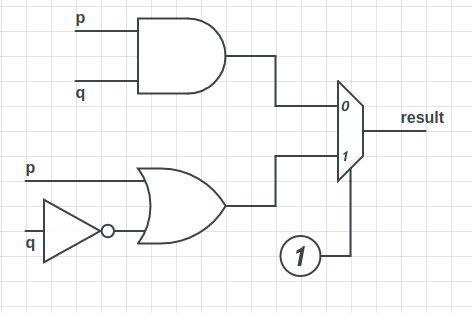
\includegraphics[scale=0.5]{circuit.png}
	\caption{Combinational Circuit}
	\label{fig: circuit}
	
\end{figure*}

In Figure \ref{fig: circuit}, the two statements are used as input. The circuit has 3 gates as AND, OR and NOT operators. It has also a 2x1 multiplexer\footnote{https://www.geeksforgeeks.org/multiplexers-in-digital-logic/} which provides to select one of the two options. 
\subproblem{a} Write the sentence that "result" output has.
\solution
\newline
\textcolor{red}{It is sunny or the flowers are not blooming.}
\newline
\newline
\subproblem{b} Convert Figure \ref{fig: circuit} to an algorithm which you can write in any programming language that you prefer (including pseudocode).
\solution
\newline
\textbf{int multiplexer; \newline
cout $<<$ "Enter the multiplexer: "; \newline
cin $>>$ multiplexer; \newline
if(multiplexer == 0) \newline
cout $<<$ "It is sunny and the flowers are blooming"; \newline
else if(multiplexer == 1) \newline
cout $<<$ "It is sunny or the flowers are not blooming"; \newline}
\newline
\newline
\end{document} 
